\chapter{Application design and implementation}
\label{chap:design}

\par In order to achieve a clear structure for the application, with layers, which provide specific services, I utilize Object Oriented Programming. It is a paradigm based on object, meaning sets of data and procedures neatly packed together. The four principles on which it is built on are encapsulation, inheritance, polymorphism and abstraction \cite{Blaschek1994}.
\par Encapsulation means that the data is bundled together in one coherent package. In the case of classes it means that the data and the methods provided to manipulate them are under one roof. The limitation on these fields are also part of the principle, providing a way to minimize the outside access to certain information if needed.  
\par Inheritance provides a way to better generalize classes, by enabling to derive the attributes and functionalities from a preexisting one. For example let's take a car, which has certain methods and variable, than we would like to create a specific version, like an Audi. In this case we can inherit all the car specific things by using inheritance, while also leaving a way for the Audi class to create new features.
\par Polymorphism is the concept of accessing multiple types of objects through one common interface. This can usually occur in two different scenarios. The first one, static, is at compile time, for example method overloading is using the same function name for multiple methods. In this case the compiler decides when to use which based on the signatures of the procedure. The second scenario, dynamic, is at runtime, when the specific type of a variable will only be known when it gets saved. For this purpose a common interface is used, be it an actual interface or a parent class, and all the objects which implement the interface or inherit the parent class, will be seen as such by the program.  
\par Abstraction is the concept of hiding unnecessary complexity from the user, by moving the implementation details under an umbrella object. For example looking at simple service, which creates a desk from different types of components, by wrapping all the implementation in one class, we hide the complexity from the end user, only needing to work with a couple of methods from the service. 

\par With the utilization of OOP, a clear architecture is achievable for the application. I use a layered architecture similar to the Model View Controller, MVC, design pattern, visible in image\ref{fig:umldiagram}.

\begin{figure}
    \centering
    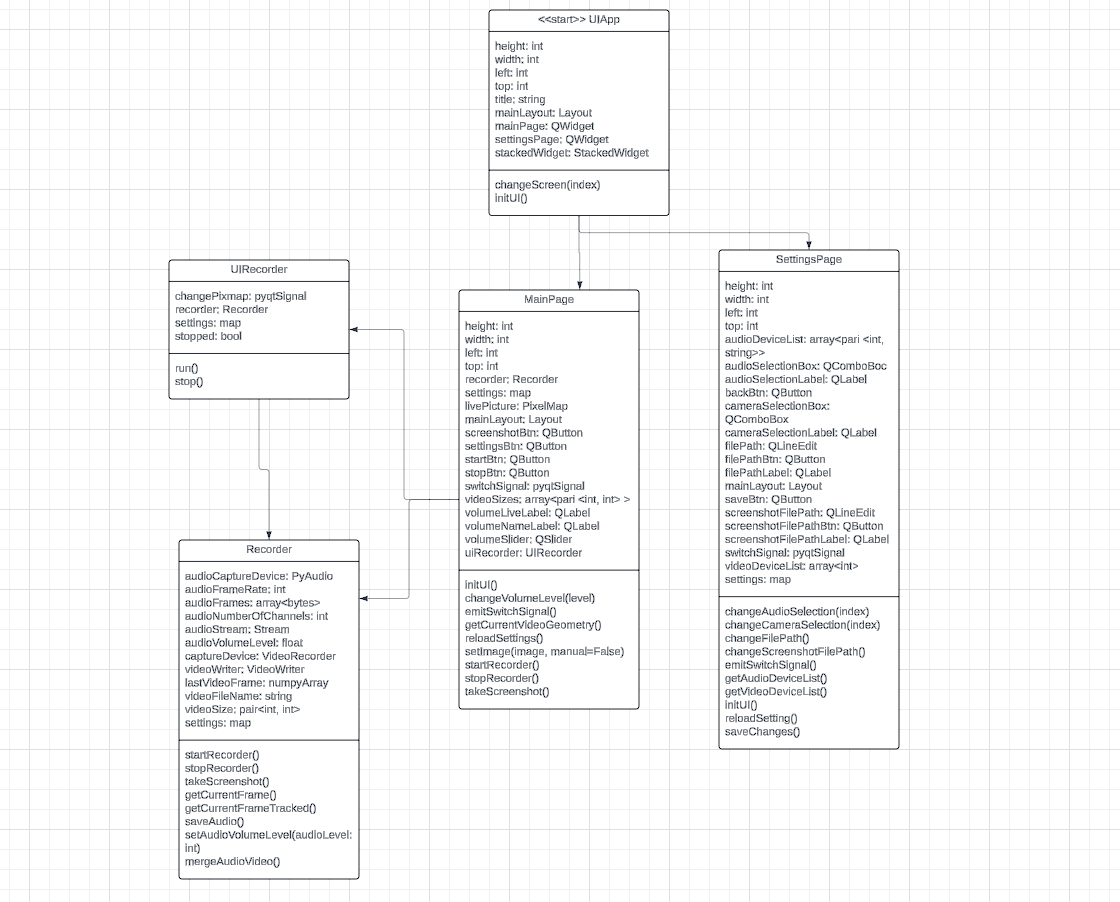
\includegraphics[width=0.8\linewidth]{figures/UML-Diagram.png}
    \caption{UML class diagram showing the relationships between the layers, made with \cite{lucidchart}}
    \label{fig:umldiagram}
\end{figure}

\par The MVC pattern is used to clearly separate the tree parts of the application for easier overview and implementation. The top layer is the view unit, be it a Graphical User Interface or any other, with which the user directly interacts with. The layer underneath is the controller one, which implements all the logical steps and calculation the application may need. It interact with the view and model layer. The last layer is the unit responsible for storing the data used, either in memory or in any other way.
\par In the case of this application the view and control layers are clearly present, with the help of a GUI and the Recorder service, see in image\ref{fig:umldiagram}. The last layer is utilized with classes from the opencv and wave modules. The VideoWriter object is used to save the captured visual footage on disk, while the wave module is for saving the audio in file. To not create another class just for wrapping this modules, resulting in some decrease in performance, I opted to leave this part in this layer. Besides this, there is also a one frame buffer present, storing the last captured visual frame. It is made in this layer for simplicity, since it is used for the screenshot functionality, creating the model layers, would just result in efficiency loss and more boilerplate code. 
\par In the second layer, which contains the Recorder class, I utilize the facade design pattern \cite{facade}. The main premise of it is that more complex systems are hidden away from the end user, providing a more simple platform to work with. From the methods shown in image\ref{fig:umldiagram}, the four methods called from the view layer are the start, stop and get frame function, all of them providing the more complex system, such as saving the video files, creating and utilizing the model layer objects and taking advantage of the Machine Learning model.
\par The three way relationship between the MainPage, UIRecorder and Recorder is discussed in the next chapter \ref{sec:designsec1}

\section{Graphical User Interface}
\label{sec:designsec1}
\par The Graphical User Interface utilizes the signal based communication of the QT framework, for inter widget discussion. This is an event based system, which allows independent objects to communicate in case when something of interest happens in the application \cite{qtSignal}. With this feature breaking the different pages down to different object altogether, making it simple for possible future additions.
\par To overcome the complexities which come with such a solution, two design patterns are used, namely the Composite and the Mediator, both of which are represented in the UI design in image\ref{fig:uidesignpattern}.

\begin{figure}
    \centering
    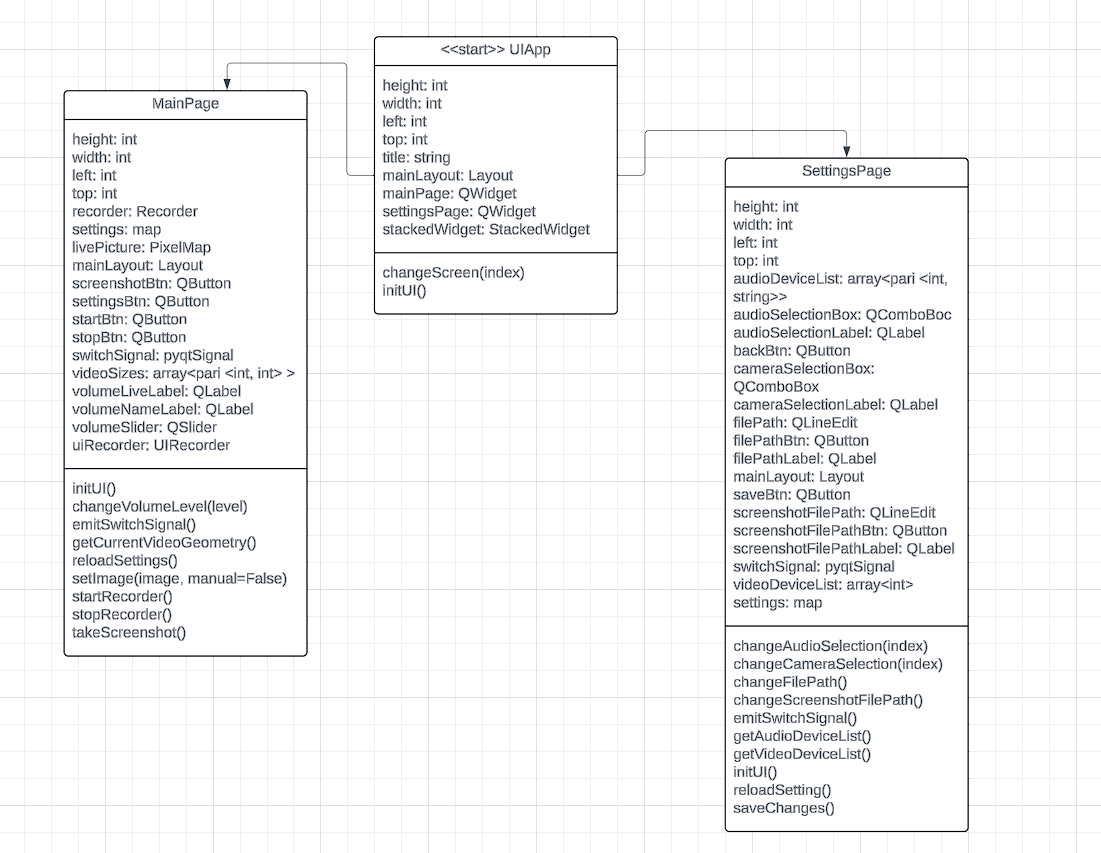
\includegraphics[width=0.8\linewidth]{figures/UIDesignPattern.png}
    \caption{Main design of the Graphical User Interface, made with \cite{lucidchart}}
    \label{fig:uidesignpattern}
\end{figure}

\par The composite design pattern states that the structure of what you are building can be represented in a tree, like a box containing more boxes and so on \cite{composite}. In the case of this application this pattern is in image\ref{fig:uidesignpattern}, in how the three widget classes are built. The main part, which is basically the control unit of the UI, the UIApp consists of the two page widget, from which the currently selected one is called to be shown.
\par The Mediator design pattern is used to keep the dependencies of different objects in check, by not letting them directly talk to each other, only through third object, the mediator\cite{mediator}. In the GUI this is done between the pages, when the switch happens between them, in the context of reloading the settings. When the switch occurs the two widget communicate with UIApp class as with their controller, since the change is not done by the pages. However in the mean time, the settings variable does need to be reloaded every time a switch occurs to ensure up-date settings at all-time, and that is where the mediator role comes in. For example when the Settings page releases control, it signals the Main page through the UIApp, the mediator, to update its settings.
\par Just how the image\ref{fig:uidesignpattern} suggest, the UIApp plays the controller role in the User Interface design, making sure the widgets are shown and that they can send each other information about the occurrences of certain events.

\begin{figure}
    \centering
    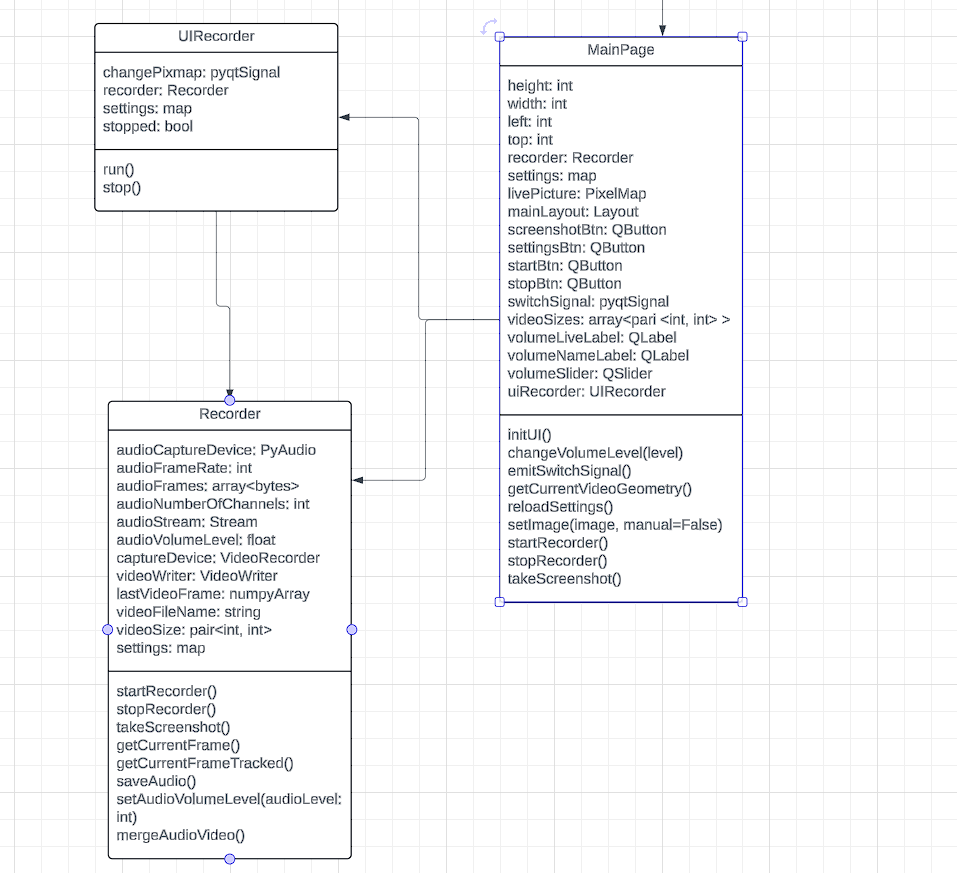
\includegraphics[width=0.8\linewidth]{figures/UIRecorder.png}
    \caption{The design of calling the controller layer in UI, made with \cite{lucidchart}}
    \label{fig:UIRecorder}
\end{figure}

\par Since the QT framework by default runs on one thread, when updating the live feed, the rest of the application becomes near unusable, since the recorder is always running. To combat this Main page, where the main functionalities can be found will not call the Recorder directly, instead creating a QThread object, UIRecorder, as can be seen in image \ref{fig:UIRecorder}.
\par Now running that the calling is done on a different thread, the returned frame has to be sent back to the Main page for visualization. For this a simplified version of the Observer design pattern is used, provided by the QT framework's signaling system. This feature allows widgets to connect to other ones in an event driven fashion. In the application the Main page will subscribe/connect to the UIRecorder's signal, changePixmap \ref{fig:UIRecorder}, and will be informed when the UIRecorder emits a signal. In this case the signal will be the new frame returned by the Recorder, enabling it to show it to the user.
\par The GUI has a minimalist look, providing the interactive elements in rows, using the Grid system of QT. In the Main page, the first row contains the live feed, the second contains the volume slider and the final row contains the navigation button Settings and the three functionality ones for starting and stopping the recording and taking a screenshot \ref{fig:MainPage}.

\begin{figure}
    \centering
    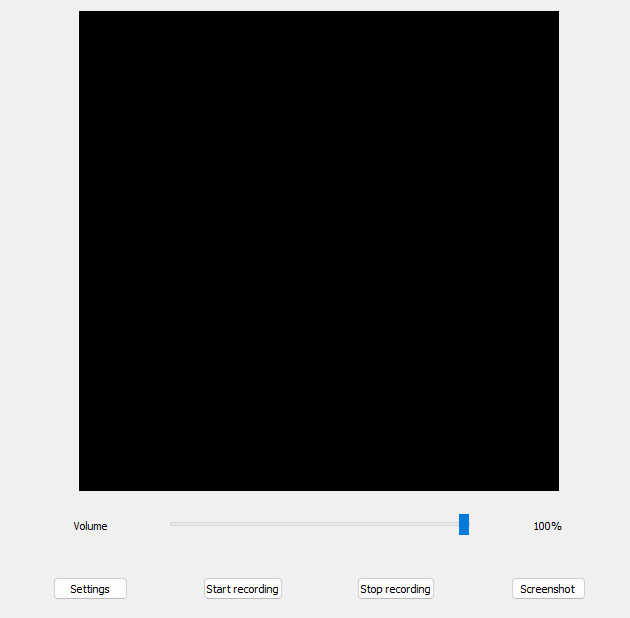
\includegraphics[width=0.5\linewidth]{figures/MainPage.png}
    \caption{The layout of the main page}
    \label{fig:MainPage}
\end{figure}

\par The Setting page is built with the same design in mind. The different sections occupy two rows each and are horizontally centered, while the last row contains the two buttons, one for saving the changes, one for navigating back to the Main page. This design creates a minimalist horizontally look, keeping the theme from the Main page \ref{fig:SettingsPage}.

\begin{figure}
    \centering
    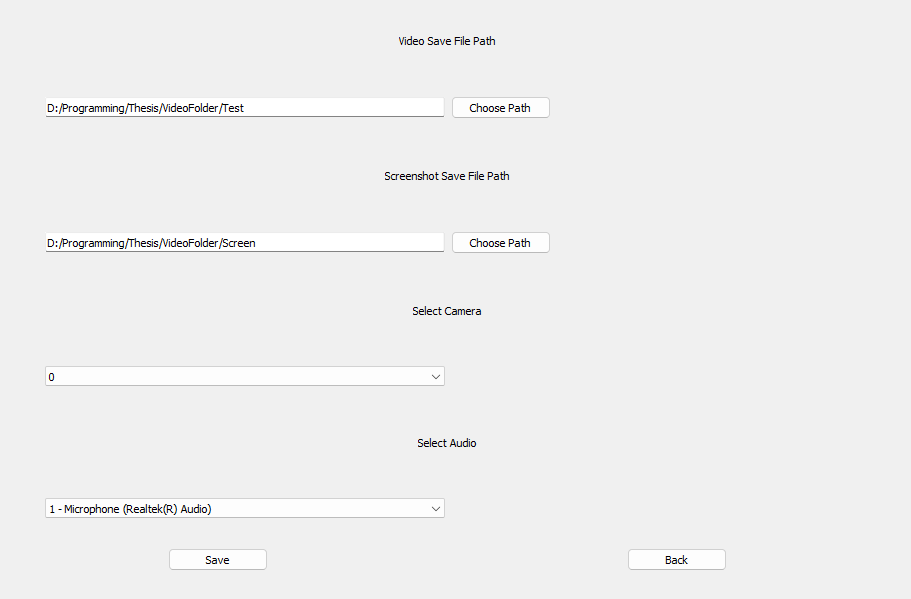
\includegraphics[width=0.8\linewidth]{figures/SettingsPage.png}
    \caption{The layout of the settings page}
    \label{fig:SettingsPage}
\end{figure}

\section{Image processing}
\label{sec:designsec3}

\par The image processing is contained withing the Recorder object. It has two function to get the current recorded frame, a simple one and one where the deep learning model is utilized. The GUI calls the perspective model, depending on whether the AI assistance is toggle on or not. The model is loaded in this layer from the start of the application, for quicker response time when needed, than the function works with the predicted hand gesture and if needed calculates where the current drawing pixels have to placed in the image.

\section{Functionality implementation}
\label{sec:designsec2}

\subsection{F1 implementation}
\label{sec:designsec2subsec1}

\par The F1, start recording, functionality utilizes a QThread, in order to enable the Main page to function properly during video recording. In this case the UIRecorder does not communicate directly with the Main page, but through the QT provided event based signal system. Besides the multi threaded nature of this feature, the flow of the calls is still quite linear, as can be seen in image\ref{fig:F1Sequence}.

\begin{figure}
    \centering
    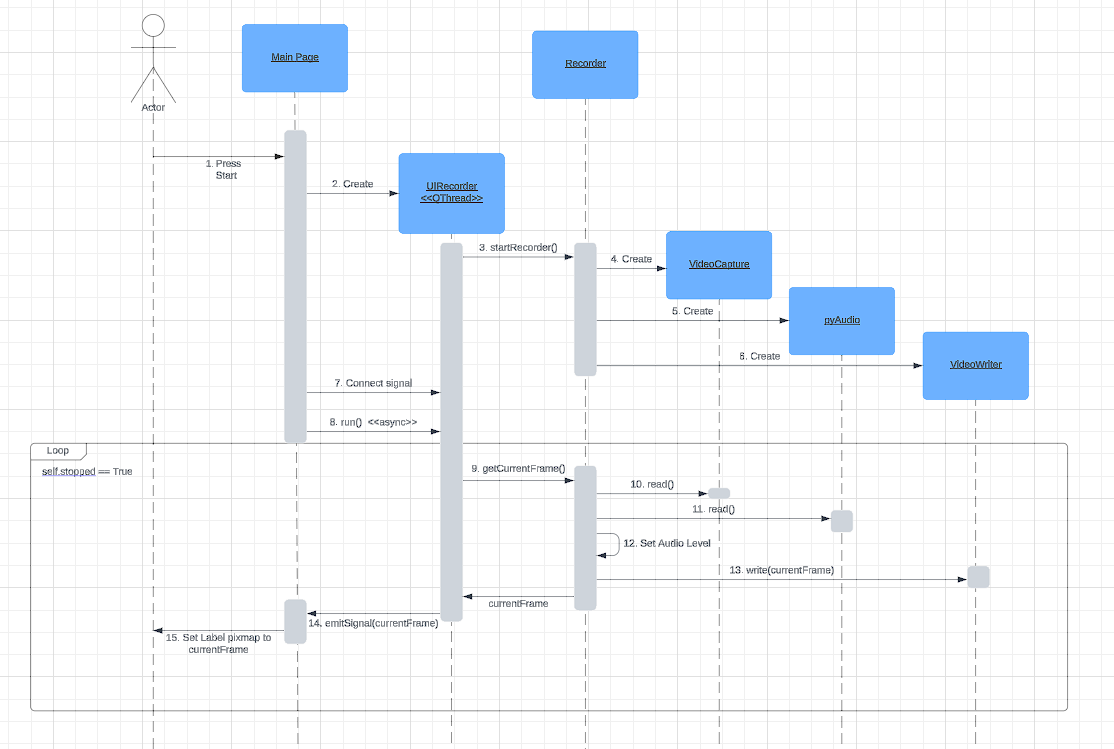
\includegraphics[width=0.8\linewidth]{figures/F1Sequence.png}
    \caption{Sequence diagram of functionality F1, made with \cite{lucidchart}}
    \label{fig:F1Sequence}
\end{figure}

\par The first step after the user hits the Start button is to set up the recording environment. To achieve this the MainPage widget will create a UIRecorder object which inherits the properties of QThread. The class saves all the parameters sent to it, like the pointer to the Recorder object and the settings map variable, than at the end of the initialization process it calls the Recorder's startRecorder function. This method will create the VideoCapture, VideoWriter and pyaudio object with the necessary configuration, couple of them being hard coded, like the number of bytes in an audio stream chunk, the rest is stored in the settings variable, like the chosen camera and microphone indexes. After the initialization of the thread is complete the MainPage widget connects its signalSlot, the setImage method, to the UIRecorder's changePixmap signal, which will be the communication channel between the two objects. And finally through an asynchronous call the MainPage widget runs the UIRecorder.
\par The running UIRecorder works in an infinite loop until the F2 functionality stops it. In this it gets the current frame by calling the getCurrentFrame or getCurrentFrameTrakced methods of the Recorder. The main premise of both of the functions is that they read the input from the VideoCapture and pyaudio object. The getCurrentFrame processes the audio by adjusting the volume level, multiplying the audio array by a float between 0 and 1. The getCurrentFrameTrakced does the same thing with the addition of processing the image with the help of the machine learning model. After the processing the write method of the VideoWriter object is called to save the visual frames to the initialized video file, than the current frame is returned to the UIRecorder. When the current frame is returned a signal is emitted though the changePixmap variable, sending the frame to the MainPage widget as a QImage object, which than sets the pixel map of the live feed label to the returned image.
\par In image\ref{fig:F1Sequence} the AI assistance free version is presented. With image processing enabled there would be two changes made, firstly the function call at step 9 would change to getCurrentFrameTrakced(), secondly there would be an extra step present between 12 and 13, called processVisualInput(). This method would be responsible for making the predictions with the help of the Deep Learning model and taking actions accordingly by manipulating the visual frames or by changing the volume level in the Recorder.